% !TeX root = ../main.tex
% Add the above to each chapter to make compiling the PDF easier in some editors.

\chapter{INTRODUCTION}\label{chapter:introduction}

It is safe to say that the internet paved the way for many things for humanity.
Media such as images, video and audio can be shared across websites and applications, knowledge can be stored on faraway servers.
This knowledge can then be retrieved with ease in text format using mobile devices, and products and services can be bought with the click of a button or a tap on a screen.
Interactions, media and information make up for massive amounts of data that flow through complex computer systems, which in turn generate even more data and information.

Researchers have found ways to leverage the magnitude of data that is being produced every second by countless systems all around the world.
One of the most recent and most popular uses of this huge variety and quantity of data is deep learning.

Recently, models such as BERT \cite{devlin2018bert}, DALL-E \cite{ramesh2021zero}, GPT-3 \cite{brown2020gpt3} and others have become incredibly popular thanks to their outstanding results and endless possibilities.
DALL-E for example can generate high-quality realistic images and art starting from a text description written in natural language.
These models however require massive amounts of data as well as very expensive computational resources, such as graphical processing units and tensor processing units (TPUs).
In recent years, the size of neural network models has been steadily increasing exponentially, as shown by \autoref{fig:model-size-over-time}.
A simple calculation shows that the neural network model Megatron-Turing-NLG 530B \cite{smith2022megatronturingnlg} would take roughly $530 \times 4 = 2120$GB of memory to simply hold its 530 billion weights.

Training a neural network model requires even more memory.
Intermediate computation outputs such as gradient and optimizer states sometimes require 2 or 3 times as much memory than just the model parameters, making GPU memory one of the main bottlenecks in training huge neural network models.
While some of these issues can be tackled using techniques such as parameter quantization \cite{DBLP:journals/corr/abs-2003-11316}, pruning and compression, they must not be considered one-fits-all solutions.
Some models are simply too big to be trained on a single device.
This problem is exacerbated by factors such as high GPU prices and much slower growth of their memory size relative to model size.
\autoref{fig:gpu-vram-over-time} shows the increase of GPU memory from 2016 to 2022.

\begin{figure}[h]
    \centering
    \caption{GPU VRAM over the past 4 years. The growth is mostly linear, doubling }
    \label{fig:gpu-vram-over-time}
    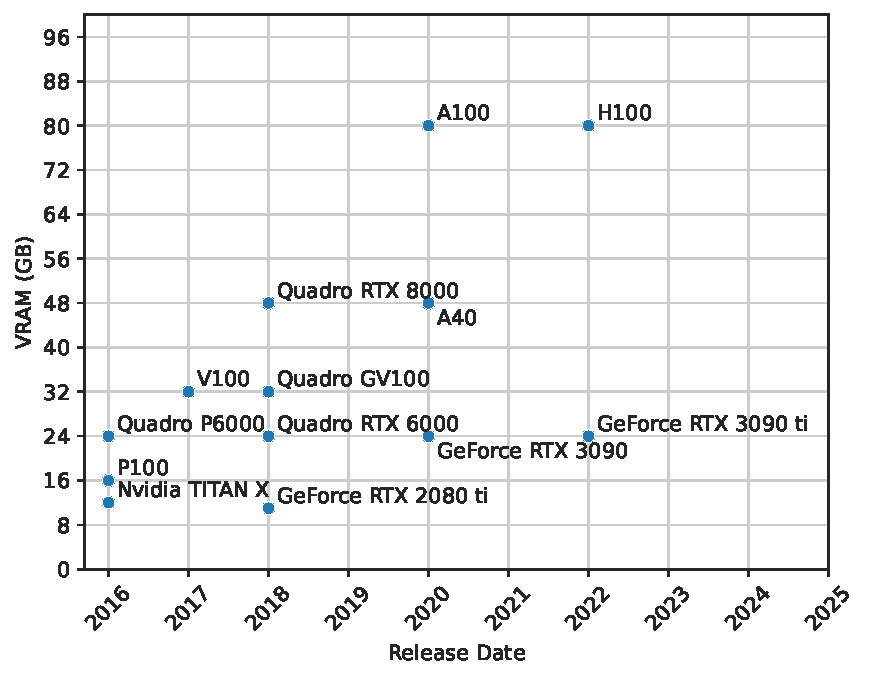
\includegraphics[width=0.75\textwidth]{./figures/gpu-vram-over-time.pdf}
\end{figure}

\begin{figure}[h]
    \centering
    \caption{Model size over the past 4 years, in logarithmic scale: ELMo \cite{peters2018elmo}, BERT \cite{devlin2018bert}, GPT-2 \cite{radford2019language}, Megatron-LM \cite{shoeybi2019megatronlm}, T-5 \cite{raffael2019t5}, Turing-NLG \cite{microsoft2020turingnlg}, GPT-3 \cite{brown2020gpt3}, Megatron-Turing-NLG \cite{smith2022megatronturingnlg}}
    \label{fig:model-size-over-time}
    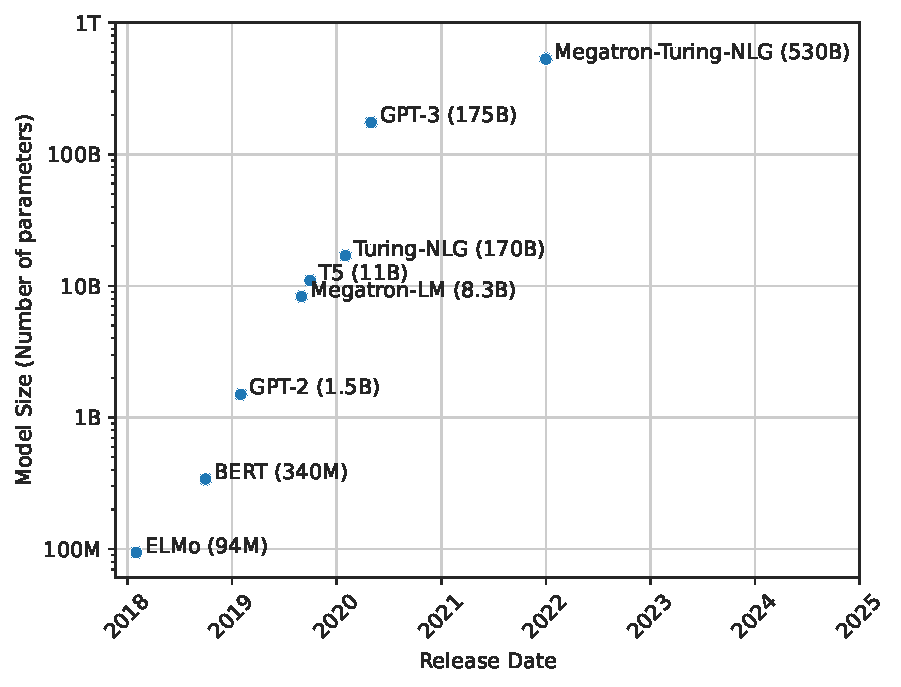
\includegraphics[width=0.75\textwidth]{./figures/model-size-over-time.pdf}
\end{figure}

To tackle these issues, practitioners studied and developed distributed computing techniques to train models that do not fit entirely in a single GPU's memory, distributing the training load to potentially thousands of devices.
Data parallelism has been widely adopted in the scientific community to train big models using paradigms such as parameter servers \cite{NIPS20141ff1de77, 10.5555/2685048.2685095} and federated learning \cite{DBLP:journals/corr/abs-1907-09693}.
Both paradigms have difficulties when dealing with heterogeneous computing nodes such as straggler nodes, synchronization and weight stalenes.
Because of this, researchers generally have to rely on massive amounts of resources and money to perform experiments and train their models using a set of homogeneous devices.
This has become a problem for universities and small companies that want to train the models described in these papers, as they do not necessarily have access to such vast amounts of resources.
Another problem is that practitioners may need to train models from scratch due to the incompatibility of their datasets with pre-trained ones, which are often trained on the most common datasets such as Imagenet \cite{deng2009imagenet} and Fashion-MNIST \cite{DBLP:journals/corr/abs-1708-07747}.

Volunteer computing is a paradigm in which people and institutions donate their idle computing resources such as laptops and other personal devices to solve hard problems.
Historically, this technique has been used to distribute hard and complex problems such as Folding@Home \cite{10.1109/IPDPS.2009.5160922}, providing 2.43 exaflops of speed during the 2019 COVID pandemic.
However, training neural networks using volunteer computing brings many challenges.
Distributing optimization algorithms such as SGD and ADAM is challenging when dealing with heterogeneous devices.
Participating peers may drop out during training or AllReduce operations such as optimizer and model state averaging, causing issues for the whole training network.
Also, volunteer hardware may not be powerful enough to make a substantial difference in training, and in fact, their results may be discarded due to the inability of keeping up with more powerful peers.

Hivemind \cite{riabinin2020hivemind} is a framework that enables volunteer computing across the internet for neural network training.
In this thesis, we will analyze several aspects of training deep neural networks in a collaborative setting.

\section{Motivation}

Hivemind implements two fundamental training algorithms, Moshpit SGD \cite{DBLP:journals/corr/abs-2103-03239} and DeDLOC \cite{DBLP:journals/corr/abs-2106-10207}.
Moshpit SGD focuses on dealing with peers that may drop out during training, excluding their collaboration from the calculation if they become unavailable or unreliable.
The focus of DeDLOC is instead on adapting the roles of participating volunteers depending on the current state of training.
Hivemind allows enabling several other distributed training features, such as large batch training \cite{goyal2017accurate} and controlling when averaging steps should be performed.
The authors experimented with the tool in a real-life scenario by training a modified version of DALL-E \cite{ramesh2021zero} with 40 peers for two months \cite{learning30:online}.
Most of the participating peers have donated their computing power through free resources such as Google Colab or their own hardware.

Although Hivemind was designed with internet training in mind, it can still be used to train neural networks within the perimeter of a single institution in controlled environments.
We think that Hivemind can help researchers leverage their currently available hardware to perform training on large neural networks, instead of buying new and more expensive hardware.

To do so, we would like to answer the following research questions:
\begin{itemize}
    \item Is it worth to setup and using low-power devices for training with Hivemind?
    \item Is adding more nodes to the computation always good, given the same amount of computational power in total?
    \item What is the effect on loss and training of increasing the number of gradient accumulation steps?
    \item What is the effect on loss and training of enabling Hivemind local updates?
\end{itemize}

In this thesis, we show that training with Hivemind in a controlled environment using limited and less powerful resources is still possible, with a few caveats and tuning.

\section{Approach}

To answer the questions above, we created 288 experiments performed on ResNet18 \cite{he2015deep} model trained on Imagenet-1k \cite{deng2009imagenet} and compile a lessons-learned section.
In this thesis, we will compare regular training using a single node with 16vCPUs to training using Hivemind with multiple peers, where the sum of vCPUs per peer always amounts to 16.
Also, we use a limited sample budget for every experiment of 320,000 samples in total split across the participant nodes or rounded up to the nearest digit if the number of samples cannot be precisely split.
We compare training with key Hivemind settings, namely:
\begin{itemize}
    \item batch size (BS);
    \item learning rate (LR);
    \item number of peers involved in the training (NoP);
    \item target number of samples that must be globally reached by all peers to perform an averaging round (TBS);
    \item number of steps to accumulate gradients for before calling the optimizer step (GAS);
    \item applying the gradients at every step or accumulating them until the next averaging round using Hivemind (LU);
\end{itemize}

As we test the software and its limitations, we might find possible areas of improvement in Hivemind.
Whenever possible, we will further contribute using the knowledge gathered through our experiments by improving the Hivemind \cite{hivemind} source code.

\section{Contributions}

Our contributions are summarized as follows:
\begin{itemize}
    \item We analyze the challenges of distributed training using Hivemind and provide insights on possible improvements.
    \item We verify the effectiveness of Hivemind for different peer hardware configurations.
    \item We use the gained knowledge and insights to contribute to the Hivemind open-source library.
\end{itemize}
